% \section{Integrando el dataset Físico-Químico y el Genómico}

En este capítulo unimos los dos conjuntos de variables para evaluar si la integración de ambos datasets representan una mejora frente a los resultados de los modelos Genómico y Físico-Químico por separado. A este nuevo dataset lo denominamos dataset Integral. Las variantes usadas fueron nuevamente las encontradas en la tabla Humsavar. 

\section{Creación del dataset Integral}

El dataset Integral posee 68,508 variantes. Este número equivale a la cantidad de variantes del dataset Físico-Químico, y esto se debe a que conservamos todas sus variantes sumando variables del Dataset Genómico (ver figura \ref{fig:interseccion_integral}). Esto da un total de 64 variables, que son las variables sumadas de los datasets Genómico (14), Físico-Químico (49) y la variable de respuesta.  

\begin{figure}[H]
    \centering
    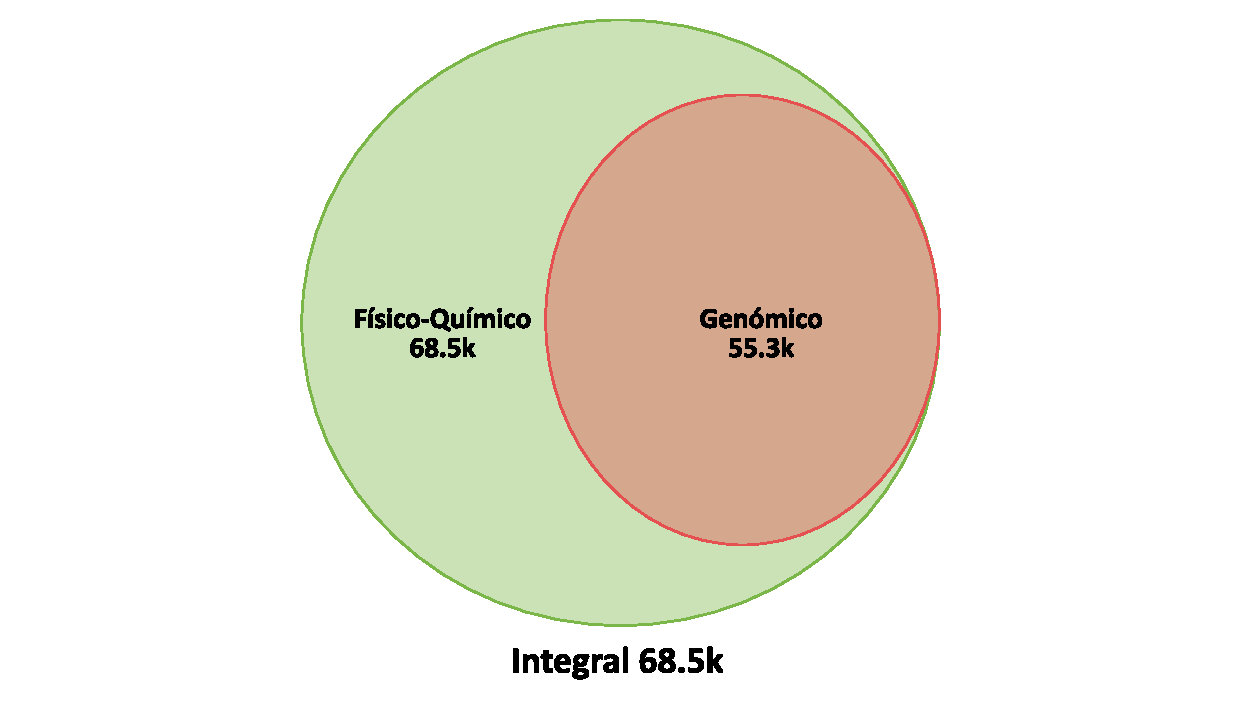
\includegraphics[scale=0.6]{documents/latex/figures/3/integral/interseccion_integral.pdf}
    \caption{Intersección entre los datasets Genómico y Físico-Químico.}
    \label{fig:interseccion_integral}
\end{figure}

Del total de las variantes, 39,653 (58\%) son benignas y 28,855 (42\%) son patogénicas. Con respecto a los nulos, mantenemos la misma cobertura de las variables físico-químicas del dataset homónimo (aproximadamente 35\% para las variables categóricas y una cobertura mayor del 60\% para las continuas), mientras que para las variables genómicas tenemos alrededor de un 20\% de variantes que no poseen cobertura al no tener un identificador rsID.

\section{Generación del modelo}

\subsection{Random Forest}

Para este modelo preliminar utilizamos nuevamente el Pipeline Tree, repitiendo las mismas fases de imputación y entrenamiento usadas previamente en los modelos Genómico y Físico-Químico. Esto significa que en la fase de imputación usamos la mediana para los valores nulos de las variables continuas y el valor más frecuente en las variables categóricas. El entrenamiento consistió en una búsqueda de hiperparámetros óptimos usando \textit{GridSearch} en un diccionario de posibles parámetros (ver sección 7.3 del apéndice), evaluados en una triple validación cruzada basándonos en el AUC como métrica a optimizar. El dataset de entrenamiento posee 45,900 variantes, aproximadamente dos tercios del dataset completo. Una vez entrenado el modelo usando este \textit{pipeline}, se evaluaron las variantes del dataset de testeo, es decir, el tercio restante del dataset completo. 

\subsection{XGBoost}

Posteriormente introducimos un método de boosting, XGBoost, nuevamente usando el Pipeline Tree. Los hiperparámetros de este método fueron elegidos usando una búsqueda randomizada (\textit{Randomized Grid-Search}). Este método de optimización fue elegido dado que las combinaciones que se evalúan en el método Grid Search son demasiadas (ver sección 7.3 del apéndice para diccionario completo de hiperparámetros explorados). La búsqueda randomizada evalúa las mismas alternativas pero eligiendo combinaciones de forma aleatoria, sin probar todas las combinaciones. También es posible evaluar valores tomados de acuerdo a una distribución específica. Decidimos dejar este análisis para trabajos futuros.

\section{Resultados del modelo Integral}

\subsection{Modelo usando Random Forest}

El modelo Random Forest obtuvo un AUC de 0.88 (ver figura \ref{fig:auc_integral}). Esto representa una mejora con respecto al modelo Genómico (0.85) y al modelo Físico-Químico (0.72). Los hiperparámetros escogidos fueron: profundidad del árbol 7 (\texttt{max\_depth}), una cantidad máxima de variables del 20\% de las variables predictoras (\texttt{max\_features}) y 100 árboles (\texttt{n\_estimators}).
Si comparamos las métricas obtenidas en el modelo Genómico con las de este modelo (ver tabla \ref{tab:metrics_integral_rf}), se puede apreciar un nuevo salto en el Recall de las variables patogénicas, que pasa de un 0.64 en el modelo Genómico al 0.80, lo que representa un 25\% de mejora. También mejora la precisión con respecto a la detección de esta clase, que pasa de 0.69 a 0.76. La única métrica que decae es el Recall de la clase Benigna, que pasa de 0.87 a 0.82, lo que representa una leve caída del F1-score. 

\begin{table}[H]
\centering
\begin{tabular}{|l|l|l|l|}
\hline
Clase        & Precisión & Recall & F1-score \\ \hline
Benignas     & 0.85      & 0.82   & 0.83     \\ \hline
Patogénicas  & 0.76      & 0.80   & 0.78     \\ \hline
Promedio     & 0.81      & 0.81   & 0.81     \\ \hline
\end{tabular}
\caption{Reporte de métricas del modelo Random Forest usando el dataset Integral.}
\label{tab:metrics_integral_rf}
\end{table}


\subsection{Modelo usando XGBoost}

El modelo XGBoost superó la performance de Random Forest alcanzando un AUC de 0.90. Las otras métricas (Precisión, Recall, F1-score) también fueron levemente superiores en todos los casos, tanto para variables benignas como patogénicas (ver tabla \ref{tab:metrics_integral_xgb}). Los hiperparámetros obtenidos en el \textit{Randomized Grid-Search} fueron:

\begin{itemize}
    \item \texttt{min\_child\_weight}: 5
    \item \texttt{gamma}: 5
    \item \texttt{subsample}: 0.8
    \item \texttt{colsample\_bytree}: 0.8
    \item \texttt{max\_depth}: 5
\end{itemize}

Utilizando el test de DeLong para comparar los AUCs del modelo RF y XGB obtuvimos un p-valor igual a $2\mathrm{e}{-16}$. Esto indica que las diferencias observadas en los valores de AUC pueden deberse a fluctuaciones aleatorias con probabilidad menor a $2\mathrm{e}{-16}$.

\begin{table}[H]
\centering
\begin{tabular}{|l|l|l|l|}
\hline
Clase        & Precisión & Recall & F1-score \\ \hline
Benignas     & 0.86      & 0.83   & 0.84     \\ \hline
Patogénicas  & 0.78      & 0.82   & 0.80     \\ \hline
Promedio     & 0.83      & 0.82   & 0.82     \\ \hline
\end{tabular}
\caption{Reporte de métricas del modelo XGB usando el dataset Integral.}
\label{tab:metrics_integral_xgb}
\end{table}

\subsection{Comparación entre los modelos}

En la tabla \ref{tab:metrics_model_integral} comparamos la Precisión, el Recall y el AUC, los tiempos de entrenamiento y de evaluación. Los tiempos de entrenamiento incluyen todas las variantes del set de entrenamiento, usando 3 folds en la etapa de validación y la búsqueda de hiperparámetros. El tiempo de evaluación equivale al tiempo de todas las variables del set de evaluación. Las métricas están basadas en las variantes patogénicas como variantes positivas. El modelo XGB supera al modelo RF en casi todas las métricas exceptuando al tiempo de entrenamiento, que incluso usando el método de busca de hiperparámetros randomizado resultó ser mucho más lento que el modelo RF, si bien es posible reducir aún más el espacio de búsqueda. Esto se debe mayormente a que a diferencia de RF que genera estimadores de forma paralela, XGB es iterativo, lo que ralentiza el proceso. 

\begin{table}[H]
\centering
\begin{tabular}{|l|l|l|l|l|l|l|}
\hline
Modelo & Precisión & Recall & AUC & F1-score & $t_{fit}$ & $t_{pred}$ \\ \hline
RF & 0.76 & 0.80 & 0.88 & 0.78 & 2m 2 s & 0.3 s \\ \hline
XGB & 0.78 & 0.82 & 0.90 & 0.80 & 12m 47s & 1.14 s \\ \hline
\end{tabular}
\caption{Comparación de métricas de modelos usando el dataset Integral. Las variables $t_{fit}$ y $t_{pred}$ corresponden al tiempo de entrenamiento y de predicción de todas las variantes}
\label{tab:metrics_model_integral}
\end{table}

\section{Importancia de las variables}

Al combinar los dos datasets Genómico y Físico-Químico volvimos a evaluar la importancia de las variables en los modelos, dado que las nuevas interacciones entre ellas pueden haber modificado los resultados anteriores. 

Si analizamos solamente la importancia usando el método de \texttt{scikit-learn} para el modelo RF (ver figura \ref{fig:importances_integral_rf}), nuevamente encontramos en primer lugar a las variables de conservación genómicas (PHYLOP46WAY y PHASTCONS46WAY), resultado esperable dado su nivel de importancia en el dataset Genómico y su nivel de AUC conseguido. También encontramos en un segundo escalón a las variables de conservación a nivel de exones, y a una variable que considera el número de SNPs en el exón donde ocurre la mutación. Luego encontramos al grupo de matrices de sustitución de aminoácidos (EX, GRANTHAM, BLOSUM y PAM250), que también aparecieron en los primeros lugares en el modelo Físico-Químico. Por último encontramos una variable relativa a la clase funcional a nivel genómico (MISSENSE) y otra relativa al cambio de polaridad del aminoácido donde ocurre la variante (POLARITY) y a la hidrofobicidad del aminoácido (HYDROPHOBICITY), por lo que encontramos en nuestro ranking una lista de variables transversal a los dos datasets usados. 


En las figuras \ref{fig:importance_cluster_integral_rf} y \ref{fig:importance_cluster_integral_xgb} unimos las variables de alta correlación en clusters y comparamos su impacto en la precisión del modelo usando la herramienta \texttt{rfpimp}. Notamos que la importancia de CONS se ve disminuida en el modelo XGB con respecto al modelo RF.


% \begin{figure}[H]
%     \centering
%     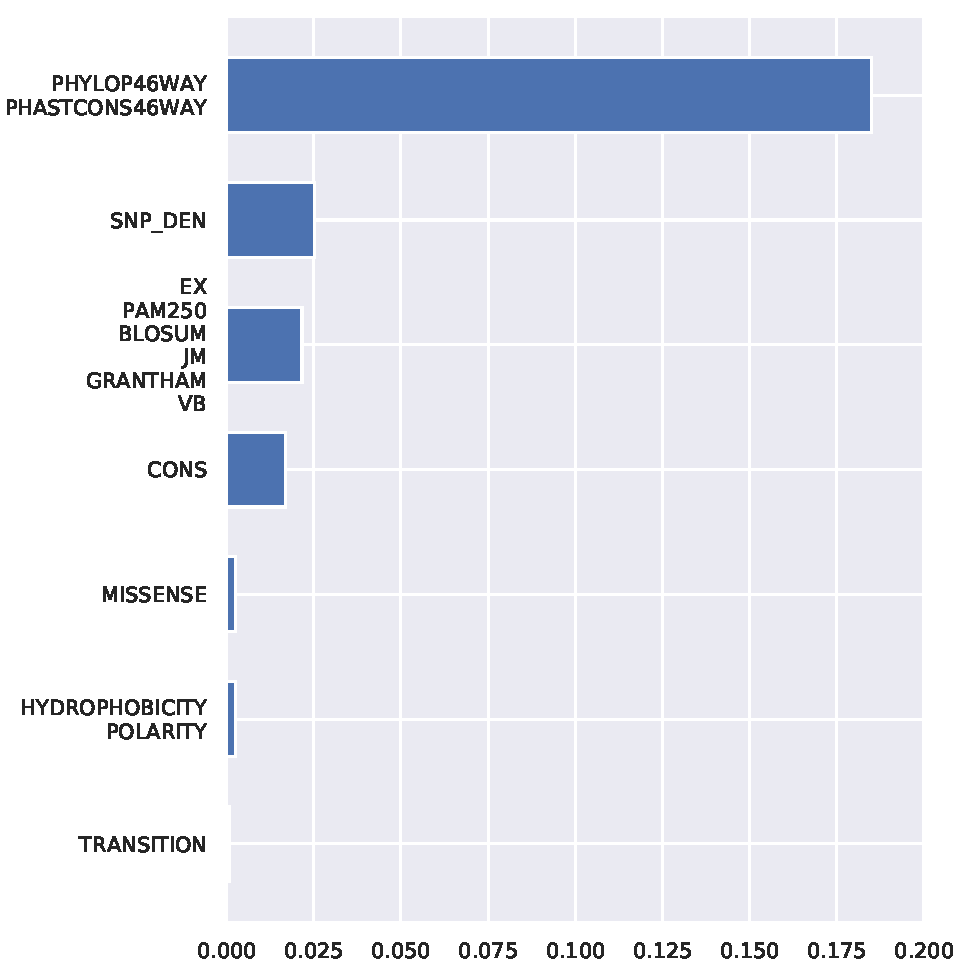
\includegraphics[scale=0.6]{documents/latex/figures/3/integral/integral_importance_cluster.pdf}
%     \caption{Importancia de variables altamente correlacionadas (basados en correlación de Spearman) usando permutación. Resultados del modelo usando Random Forest.}
%     \label{fig:importance_cluster_integral_rf}
% \end{figure}



% \begin{figure}[H]
%     \centering
%     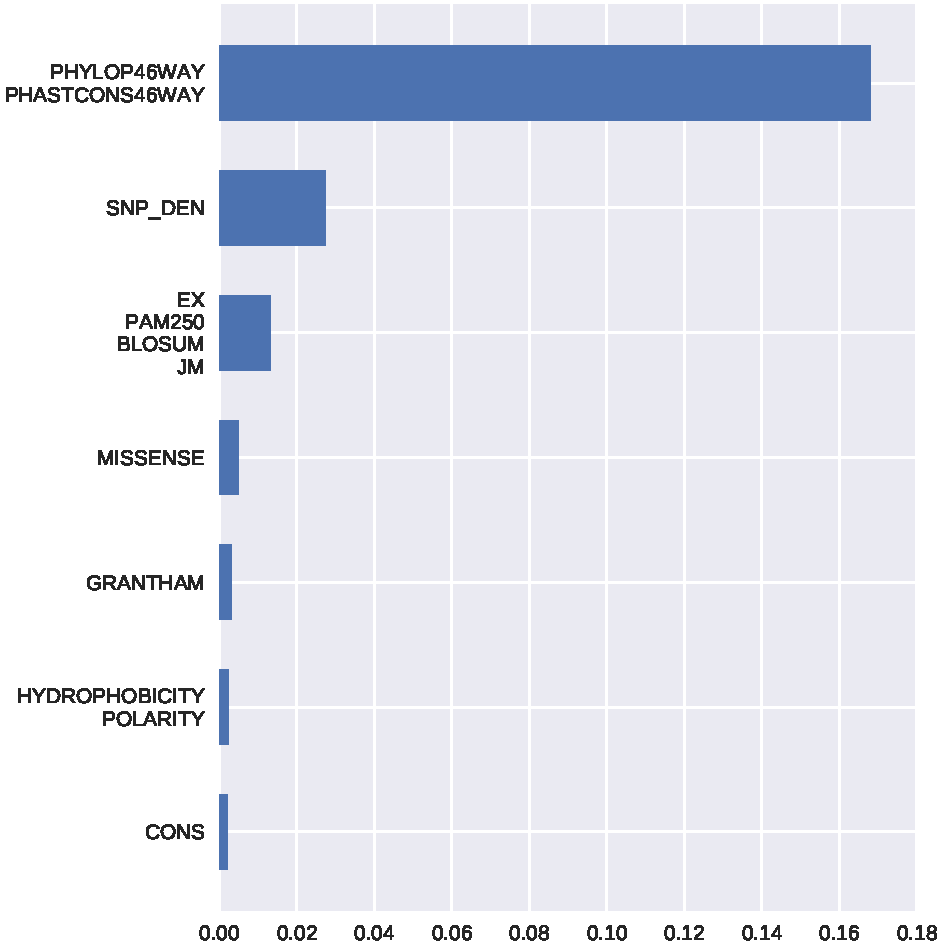
\includegraphics[scale=0.6]{documents/latex/figures/3/integral/integral_importance_cluster_xgb.pdf}
%     \caption{Importancia de variables altamente correlacionadas (basados en correlación de Spearman) usando permutación. Resultados del modelo usando XGB.}
%     \label{fig:importance_cluster_integral_xgb}
% \end{figure}

% Side by side figures 
\begin{figure}[H]
\begin{subfigure}[c]{0.45\linewidth}
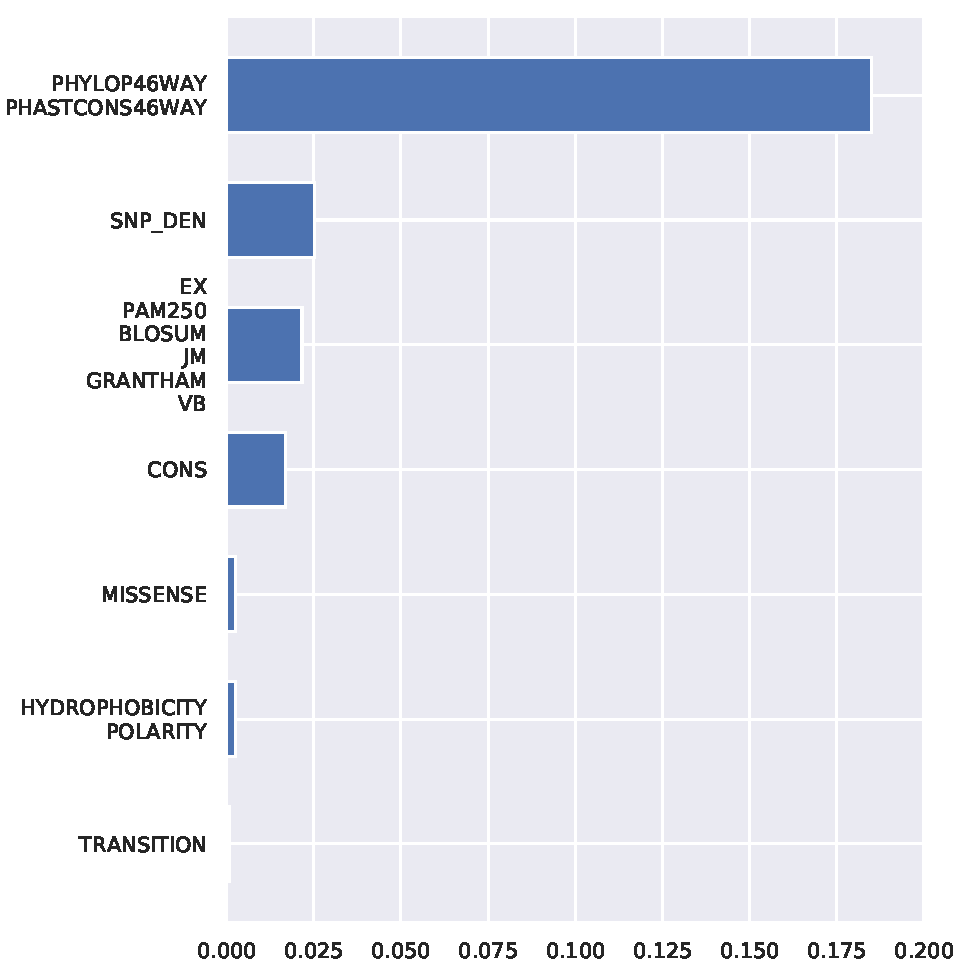
\includegraphics[width=\linewidth]{documents/latex/figures/3/integral/integral_importance_cluster.pdf}
\caption{Resultados del modelo usando RF.}
\label{fig:importance_cluster_integral_rf}
\end{subfigure}
% \hfill
\begin{subfigure}[c]{0.45\linewidth}
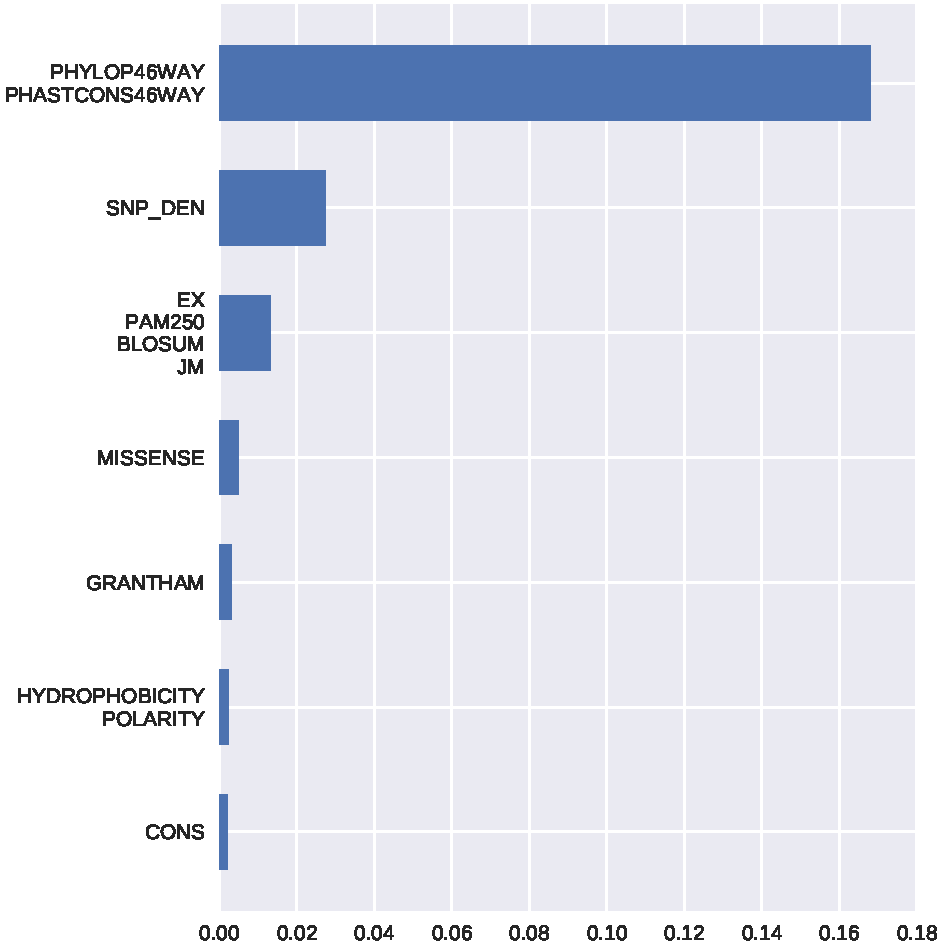
\includegraphics[width=\linewidth]{documents/latex/figures/3/integral/integral_importance_cluster_xgb.pdf}
\caption{Resultados del modelo usando XGB.}
\label{fig:importance_cluster_integral_xgb}
\end{subfigure}%
\caption{Importancia de variables altamente correlacionadas del dataset Integral (basados en correlación de Spearman) usando permutación.}
\end{figure}

\section{Conclusión del capítulo}

Como conclusión de este capítulo, resaltamos la mejora aportada tanto por el dataset Físico-Químico como por el algoritmo XGBoost. Por un lado, mantuvimos constante el algoritmo usado en la sección anterior, Random Forest, al que incluimos nuevas variables, y eso significó un salto en el AUC de 0.85 a 0.88. En un segundo paso, modificamos el algoritmo manteniendo las mismas variables, consiguiendo un AUC de 0.90. Consideramos que igualmente hay espacio para mejorar aún más, y evaluaremos la incorporación de variables estructurales en el próximo capítulo siguiendo el mismo esquema. 


% \begin{figure}[H]
% \begin{subfigure}[b]{0.5\textwidth}
%     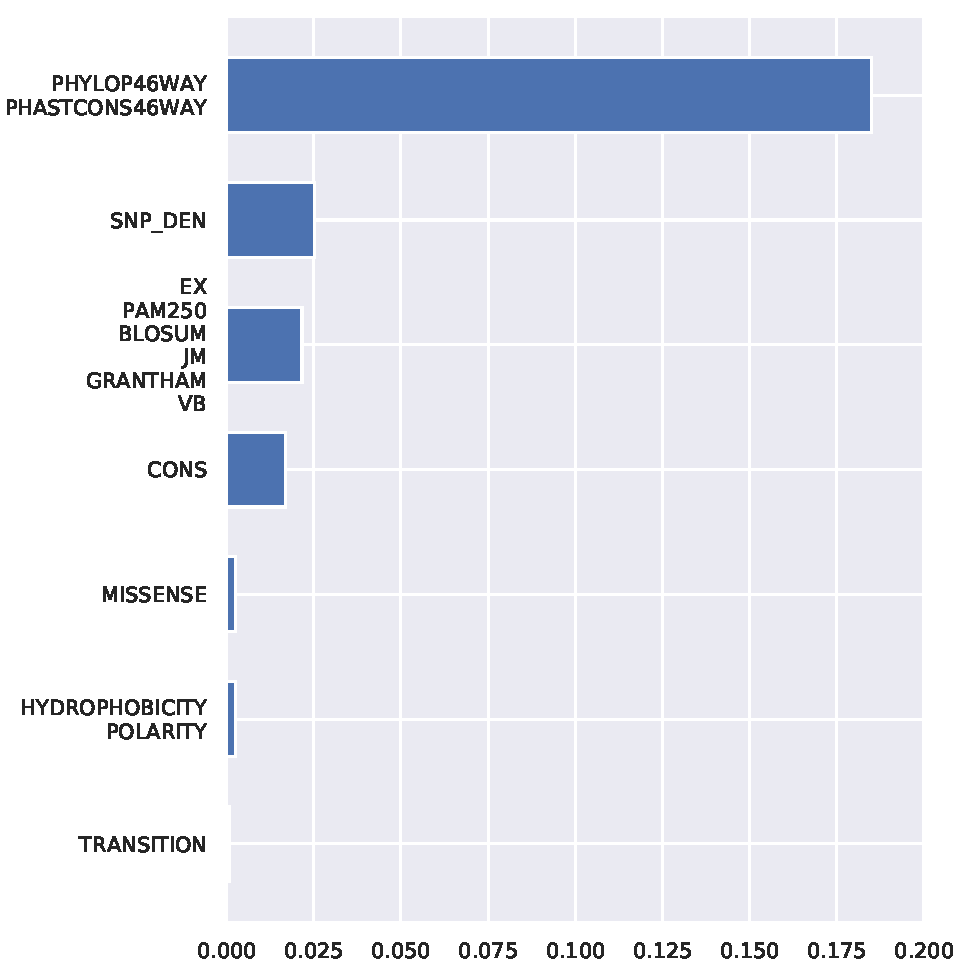
\includegraphics[width=\textwidth]{documents/latex/figures/3/integral/integral_importance_cluster.pdf}
%     \caption{Importancia de variables clusterizadas (basados en correlación de Spearman) usando permutación. Resultados del modelo usando Random Forest.}
%     \label{fig:importance_cluster_integral_rf}
% \end{subfigure}
% \hfill
% \hfill
% \begin{subfigure}[b]{0.5\textwidth}
%     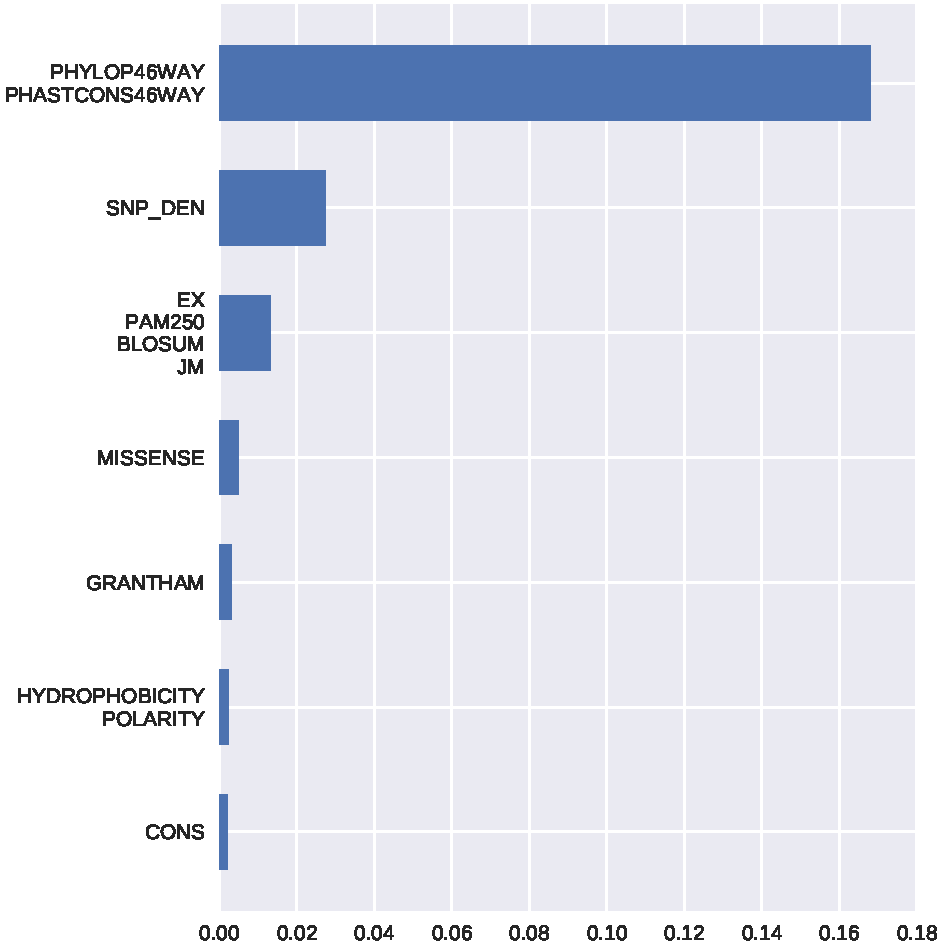
\includegraphics[width=\textwidth]{documents/latex/figures/3/integral/integral_importance_cluster_xgb.pdf}
%     \caption{Importancia de variables clusterizadas (basados en correlación de Spearman) usando permutación. Resultados del modelo usando XGB.}
%     \label{fig:importance_cluster_integral_xgb}
% \end{subfigure}

% \end{figure}





\newpage

\begin{figure}[H]
\centering
\begin{subfigure}[t]{0.7\textwidth}
    \centering
    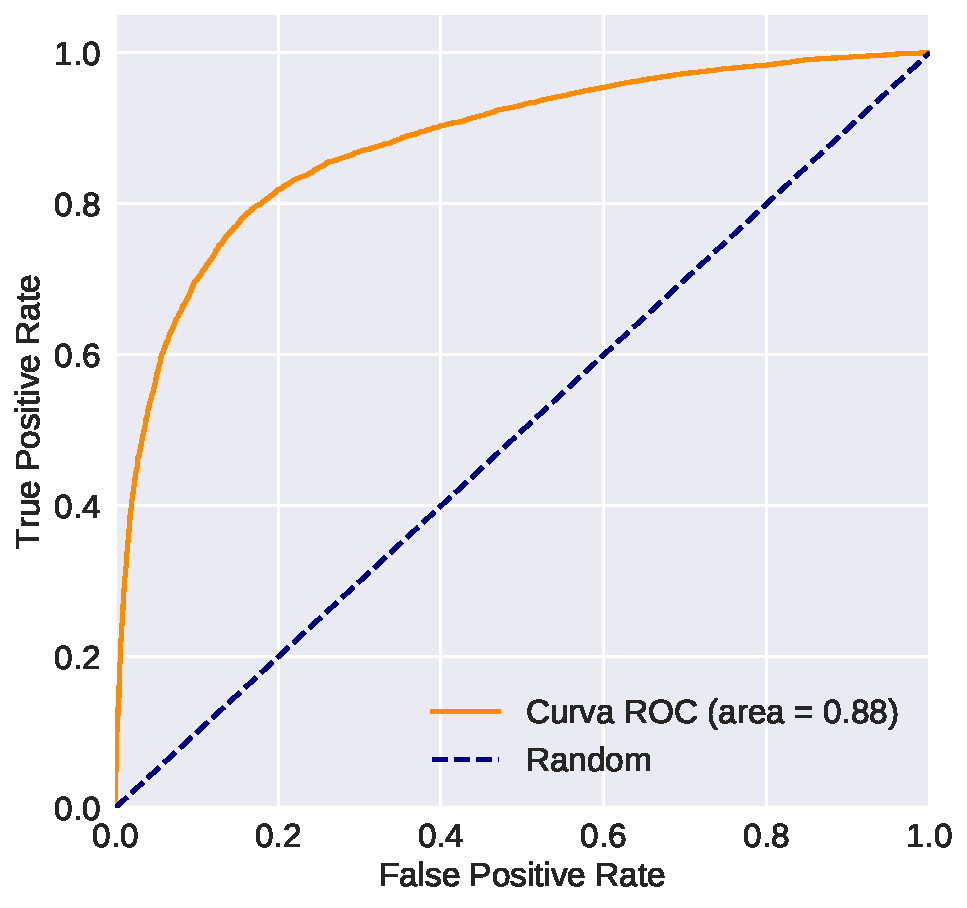
\includegraphics[width=\textwidth]{documents/latex/figures/3/integral/auc_integral.pdf}
    \caption{Comparación de curvas AUC entre algoritmos Random Forest y XGBoost. La línea punteada corresponde a un predictor Random.}
    \label{fig:auc_integral}
\end{subfigure}
\hfill
\hfill
\begin{subfigure}[b]{0.7\textwidth}
    \centering
    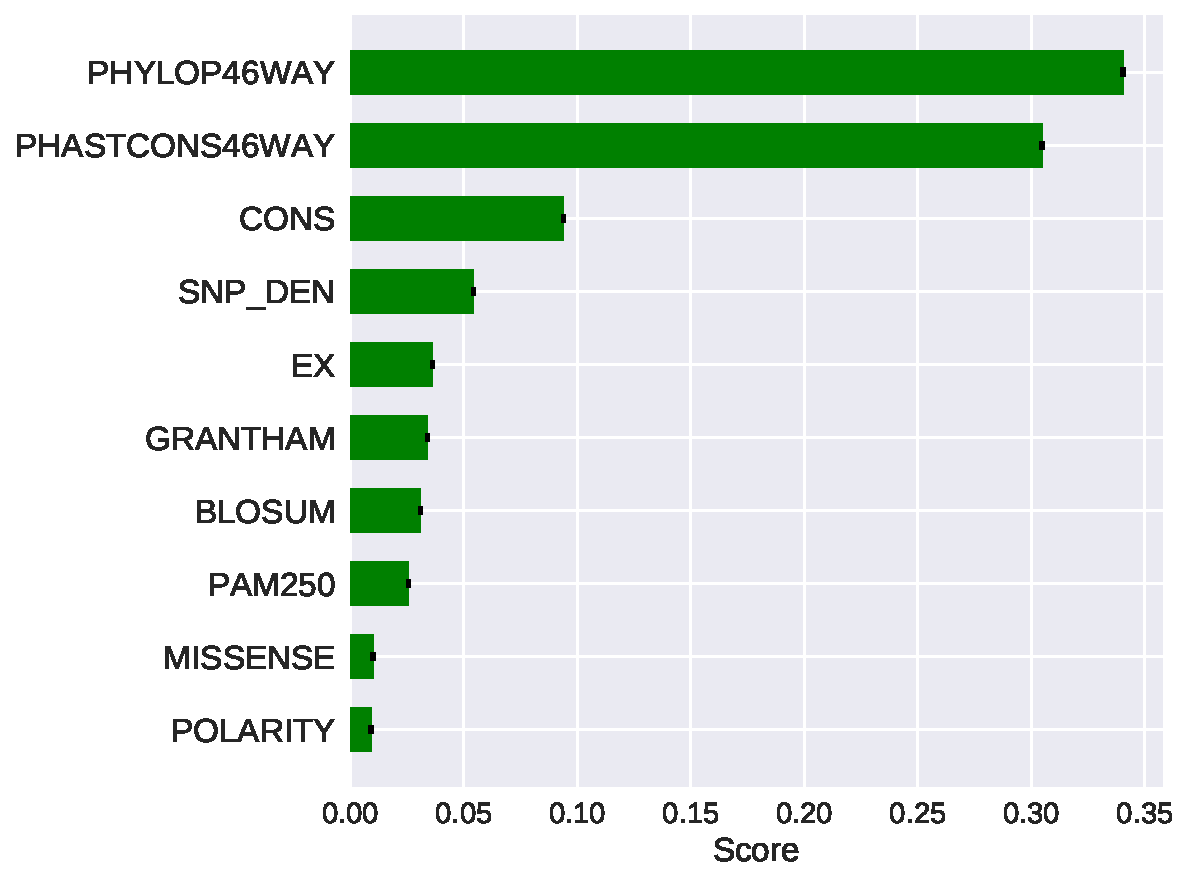
\includegraphics[width=\textwidth]{documents/latex/figures/3/integral/importances_integral.pdf}
    \caption{Los 10 atributos más importantes del dataset Integral aportados por el algoritmo Random Forest.}
    \label{fig:importances_integral_rf}
\end{subfigure}

\caption{Curva AUC y atributos más importantes de los modelos RF y XGBoost usando el dataset Integral.}

\end{figure}
